\section{问题三模型的建立与求解}

问题三在问题二的基础上引入光伏预报的日内更新：每天 0:00、6:00、12:00、18:00 均可获得未来 24 小时整点的光伏发电功率预报，微网可在 0:00 依据当时预报制定当天计划购电策略，也可在后续预报时刻调整尚未执行的购电量；计划购电量高于调整后购电量的部分按交易电价 50\% 支付违约费，调整后高于计划的部分按 1.5 倍购买。从调度与决策的角度看，问题三的本质是一个\textbf{连续决策问题}：决策者需要在“修改计划要付调整费”与“不改计划可能要买 5 倍紧急电”之间反复权衡，储能设备则每 10 分钟依据实际负荷、实际光伏与当前储能量闭环运行。因此本文采用\textbf{四阶段滚动随机规划 + 情景模型预测控制（MPC）}的整体框架：每个预报发布时刻求解一个条件两阶段随机规划，MPC 随新信息到来反复重算，四次顺序求解共同构成一条可实施的闭环策略。

\subsection{数据预处理与探索性分析}

对四份附件进行核对发现，各数据均\textbf{无缺失值、无异常值、无量纲不一致或单位错乱}，数据结构完整且相互对应，因此无需专门预处理，可直接用于建模；唯一需要注意的是附件给出的 144 个十分钟区间标签与结果模板存在十分钟错位，本文按位置对齐处理。

建模之前，我们先对负荷、光伏及二者关系作探索性分析。观察负荷数据可以发现，小区负荷呈现清晰的\textbf{日内双峰}形态（早晚两个高峰、中午凌晨较低），且\textbf{周同期}（上周同一时刻）是最强的预测线索，其加权绝对百分比误差明显低于前一日同期；这种“日内有规律、周内可借鉴”的周期性提示负荷预测应以周同期为基线。光伏出力主要由日照时长与太阳高度角决定，呈现强烈的\textbf{季节性}：夏季高峰更高、持续更长，冬季显著偏低，全年净负荷日均值在冬季约为春季两倍。将负荷与光伏相减得到净负荷后进一步发现，二者在\textbf{时间上并不匹配}——全年有近两成的十分钟时段光伏功率超过负荷、盈余集中在正午，而负荷高峰在早晚，这一错配恰恰揭示了储能“时间上的能量搬运”价值。综上，负荷的周同期周期性、光伏的季节性、以及负荷与光伏的时序错配，共同构成建模的三个关键前提。

\subsection{模型建立}

\subsubsection{符号设定与基本假设}

本文的基本假设为：一天 144 个十分钟区间、能量以 kWh 计量；问题三电价 $P_t>0$ 为附件 1 固定日内曲线；用户侧不能反向售电、光伏过剩可弃光；更新只对未开始区间生效；主口径按“最终调整量相对 0:00 原计划结算一次”；微网在每个区间内可连续计量并闭环调节。

\subsubsection{负载与光伏的因果预测}

基于探索性分析发现的周周期特性，负载预测采用“周同期基线 + 同阶段缩放”：基线取上周同一时刻负载功率 $\ell_{d-7,t}$（不足 7 天用附件 1 平均曲线），缩放系数 $a_{d,k}$ 用最近至多 36 个已观测区间的中位比例估计并以历史 5\%/95\% 分位截断，预测为 $\widehat L_{d,k,t}=\Delta\max\{0,a_{d,k}m_{d,t}\}$。光伏预测则把附件 3 的整点预报加上发布时刻实测功率作为节点，用保形分段三次插值（PCHIP）构造连续曲线并逐十分钟积分得到 $\widehat R_{d,k,t}$。所有预测严格只用当前发布时刻之前的信息，杜绝数据泄漏。

\subsubsection{联合不确定性情景}

考虑到负载与光伏的预测误差在日内高度相关，情景生成必须保留同期相关性。对历史日 $j<d$ 因果重放预测得到残差 $\varepsilon^L_{j,t}=L_{j,t}-\widehat L_{j,t}$、$\varepsilon^R_{j,t}=R_{j,t}-\widehat R_{j,t}$，再从与 $d$ 同季节的历史日中有放回抽取 $N_\omega$ 个、取同一历史日的整段残差构造情景
\begin{equation}
L^\omega=\max\{0,\widehat L+\varepsilon^L\},\qquad R^\omega=\max\{0,\widehat R+\varepsilon^R\},\label{eq:scenario3}
\end{equation}
等权概率 $\pi=1/N_\omega$。同季节条件化既反映季节差异，又避免跨季节抽样引入错误幅度的误差。

\subsubsection{供需平衡与储能模型}

对任意情景 $\omega$、区间 $t$，能量平衡与储能量递推为
\begin{equation}
G^{(k)}_{d,t}+E^\omega_{d,t}+R^\omega_{d,k,t}+D^\omega_{d,t}=L^\omega_{d,k,t}+C^\omega_{d,t}+W^\omega_{d,t},\label{eq:balance3}
\end{equation}
\begin{equation}
S^\omega_{d,t+1}=S^\omega_{d,t}+\eta_c C^\omega_{d,t}-\frac{D^\omega_{d,t}}{\eta_d}.\label{eq:soc3}
\end{equation}
式~\eqref{eq:balance3} 左边为供给侧（常规购电、紧急购电、光伏、储能放电），右边为需求侧（负载、储能充电、弃置）。由于紧急购电单价为 $5P_t$ 且常规购电无上限，最优解中紧急电只用于真实负载缺口，故单一弃置量 $W$ 即可吸收所有未利用电量而不改变最优费用。容量与功率边界为 $1200\le S^\omega_{d,t}\le10800$、$0\le C^\omega_{d,t},D^\omega_{d,t}\le\bar e\approx833.33$。

\subsubsection{计划购电与调整费用}

计划购电是非预期的第一阶段变量，对所有情景取同一值。引入绝对调整量 $A^{(k)}_{d,t}\ge0$ 满足 $A\ge G^{(k)}-G^{(0)}$ 与 $A\ge G^{(0)}-G^{(k)}$，最优时自动压到 $A=|G^{(k)}-G^{(0)}|$，从而把绝对值线性化。单区间常规购电与调整的合计费用为
\begin{equation}
\Phi^{(k)}_{d,t}=P_t G^{(k)}_{d,t}+0.5P_t A^{(k)}_{d,t},\label{eq:adjust3}
\end{equation}
经恒等变换，这与题面“上调部分按 1.5 倍、下调违约 0.5 倍”完全等价。

\subsubsection{报童下界与跨日终端价值}

规划层的第二阶段补救按情景自由取值，会高估储能的对冲能力、把计划购电量压得偏低。为对冲这一乐观偏差，对每个区间增加报童下界：计划购电量不得低于情景净负载的 80\% 分位，
\begin{equation}
G^{(k)}_{d,t}\ge Q_{0.8}\big(\{L^\omega_{d,k,t}-R^\omega_{d,k,t}\}_{\omega}\big),\label{eq:newsvendor3}
\end{equation}
其理论依据是单区间报童模型的临界比：少买 1 kWh 多付 $4P_t$、多买 1 kWh 白付 $P_t$，故最优覆盖概率为 $0.2$。

若只最小化当天费用，模型会在 24:00 前放空储能、次日丧失隔夜缓冲。为维持隔夜缓冲，构造凸分段线性终端价值 $V(s)$，在安全区间取 17 个网格点、对每个网格点用次日点预测解确定性 24 小时影子调度得未来费用，再投影到凸集合重建 $V(s)=\max\{0,\max_q(\widetilde a_q s+\widetilde b_q)\}$，并线性化为 $\theta^\omega\ge\widetilde a_q S^\omega_{d,145}+\widetilde b_q$。$\theta$ 只用于防止短视，不计入官方结算。

\subsubsection{目标函数与执行层情景 MPC}

第 $k$ 次更新时，情景 $\omega$ 的待决策成本与完整目标为
\begin{equation}
J^{M,\omega}_{d,k}=\sum_{t\in\mathcal R_k}\Big[P_t G^{(k)}_{d,t}+0.5P_t A^{(k)}_{d,t}+5P_t E^\omega_{d,t}\Big]+\theta^\omega_{d,k},\label{eq:cost3}
\end{equation}
\begin{equation}
\min\ (1-\lambda)\sum_{\omega}\pi_\omega J^{M,\omega}_{d,k}+\lambda\,\mathrm{CVaR}_\alpha(J^{M}_{d,k}).\label{eq:obj3}
\end{equation}
默认取风险中性 $\lambda=0$。由于规划层的 wait-and-see 是乐观下界，因果可实施性由执行层保证：实际运行到区间 $r$ 时，冻结已提交的 $G^F$，重采样未来情景，解“当前区间 here-and-now、未来 wait-and-see”的随机 LP
\begin{equation}
\min\ \sum_{\omega}\pi_\omega\Big[\sum_{t=r}^{144}5P_t E^\omega_{d,t}+\theta^\omega\Big],\label{eq:mpc3}
\end{equation}
只执行当前动作，并对当前区间施加互斥约束（保证不充放、紧急电不充电），下一区间重新采样重解，保持滚动因果性。

\subsection{模型求解}

规划层与执行层的目标函数均为线性函数，全部约束为线性等式或不等式，报童下界与终端价值的线性化不改变模型的线性结构，故每个子问题都是连续线性规划，可直接由线性规划求解器精确求解；本文统一采用 SciPy 的 \texttt{scipy.optimize.linprog}（HiGHS 方法）。求解按天滚动、每天四阶段顺序执行：

\begin{enumerate}
  \item \textbf{Step 1（0:00 制定原计划）}：读取当前储能量与未来 24 小时光伏预报，建立因果负载/光伏预测与联合情景，求解两阶段随机 LP，得到全天原计划 $G^{(0)}$；
  \item \textbf{Step 2（区块内闭环执行）}：进入某一 10 分钟区间前，冻结已提交的 $G^F$，重采样未来情景并求解情景 MPC，只执行当前区间的充放电与紧急购电动作，下一区间重新采样重解，保持滚动因果性；
  \item \textbf{Step 3（6:00、12:00、18:00 更新）}：冻结已执行时段，读取新预报与实测储能量，重建情景并重解剩余时域，得到更新后的总购电量 $G^{(k)}$；
  \item \textbf{Step 4（日末衔接）}：24:00 保存真实执行路径，令次日初值等于当日末储能量，返回 Step 1 推进下一天。
\end{enumerate}

四种更新策略 $M_0=\{0\},M_1=\{0,6\},M_2=\{0,6,12\},M_3=\{0,6,12,18\}$ 从同一公共初始储能量分别滚动全年，进程级并行以减小墙钟时间。

\subsection{结果分析}

\subsubsection{模型验证}

模型的正确性通过三类残差复核：能量平衡残差、储能量递推残差、费用复算残差，实测分别约 $4.6\times10^{-13}$、$9\times10^{-13}$、$3.7\times10^{-9}$，均远小于验收阈值，且无越界、无同时充放电、无紧急购电充电，说明模型求解稳定、物理口径自洽。

为评价各更新时刻的价值，本文将四种更新策略在同一公共初始储能量下分别滚动全年，比较其官方结算费用，结果如表~\ref{tab:cost3} 所示。

\begin{table}[htbp]
\centering
\caption{四种更新策略的全年官方费用（万元）}
\label{tab:cost3}
\begin{tabular}{cccc}
\toprule
策略 & 总费用 & 调整费贡献 & $\Delta C$ \\
\midrule
$M_0$（仅 0:00） & 1795.6 & --- & --- \\
$M_1$（+6:00） & 1908.1 & 110.3 & $\Delta C_6=-112.5$ \\
$M_2$（+12:00） & 1882.4 & 127.4 & $\Delta C_{12}=+25.8$ \\
$M_3$（+18:00） & 1877.6 & 126.2 & $\Delta C_{18}=+4.7$ \\
\bottomrule
\end{tabular}
\end{table}

表~\ref{tab:cost3} 显示，仅保留 0:00 计划的 $M_0$ 总费用反而最低，依次加入 6:00、12:00、18:00 更新后总费用不降反升。为看清总费用由何驱动，图~\ref{fig:q3_cost} 给出各策略的计划购电费、调整费与紧急购电费的分解。

\begin{figure}[htbp]
\centering
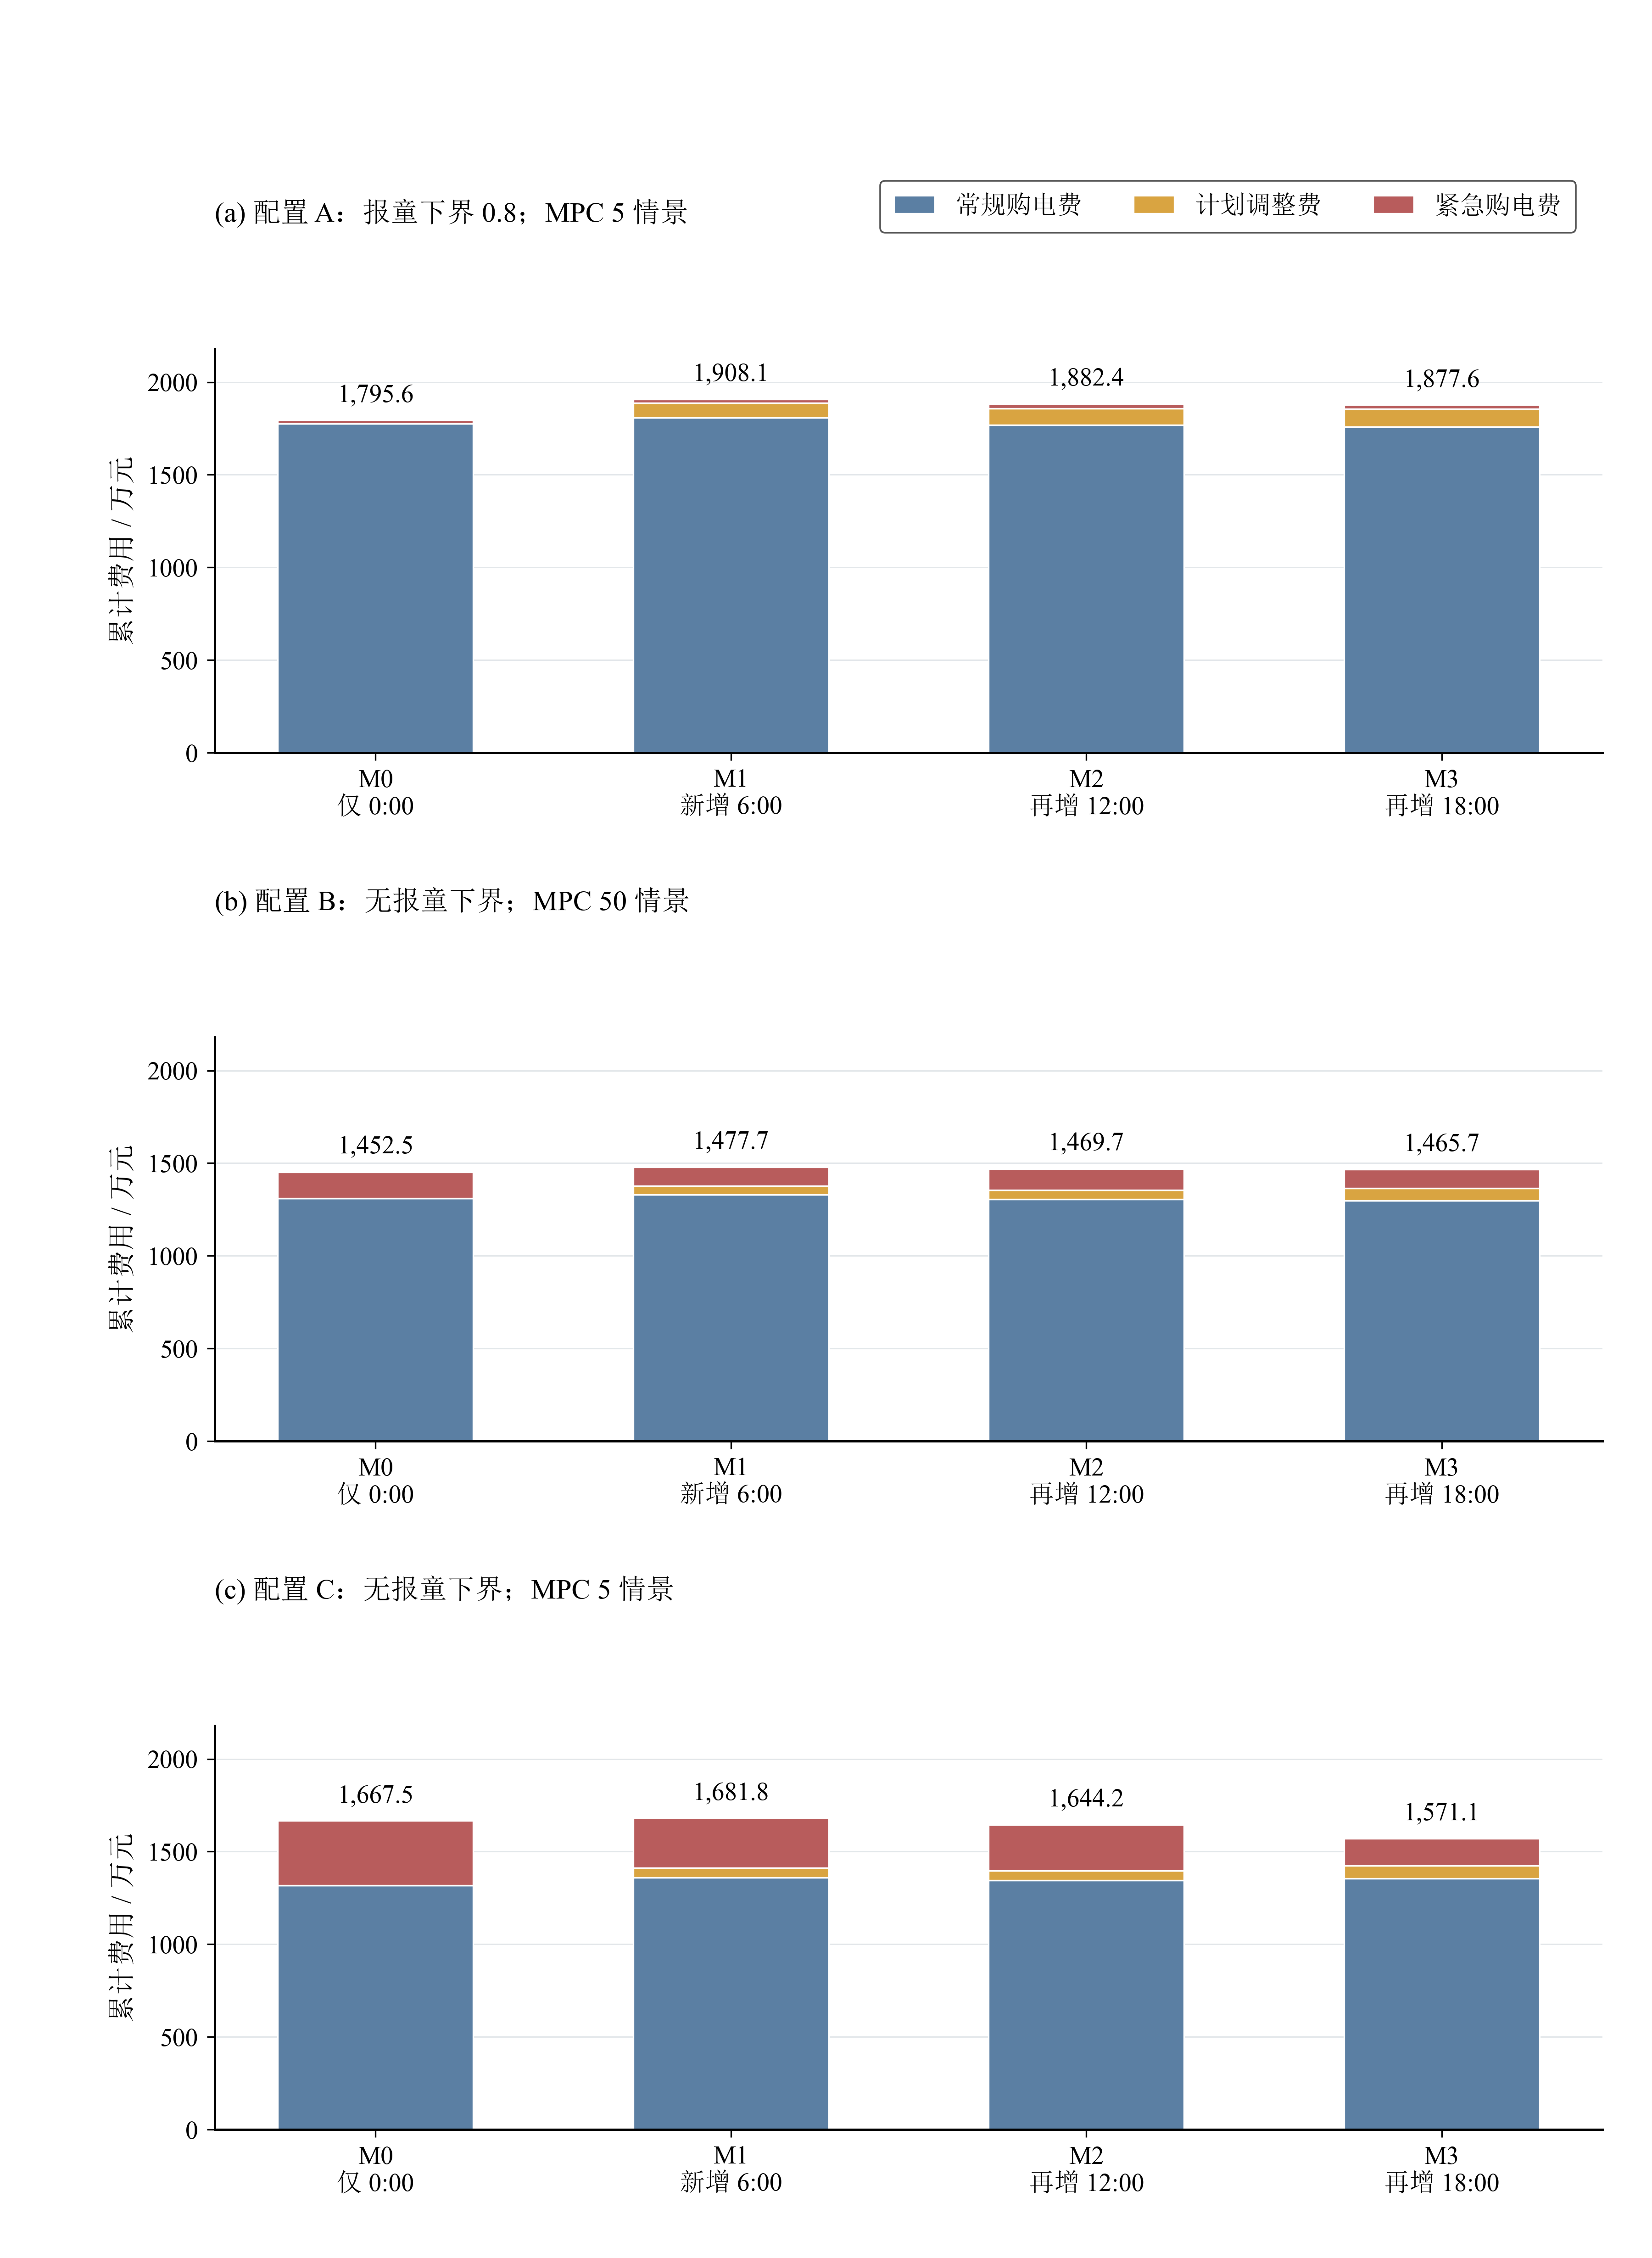
\includegraphics[width=0.50\textwidth]{figures/01_q3_cost.png}
\caption{四种策略的费用构成}
\label{fig:q3_cost}
\end{figure}

观察图~\ref{fig:q3_cost} 可以发现，四种策略的紧急购电费均处于较低水平（得益于报童下界与情景 MPC 的双重对冲），总费用主要由计划购电费主导；而 $M_1,M_2,M_3$ 相对 $M_0$ 多出的调整费，正是其总费用偏高的直接原因。这一结果提示：日内更新虽能改善计划精度，却要额外支付调整费，其经济性取决于“精度提升”与“调整代价”的权衡。

\subsubsection{关键设计取舍的敏感性分析}

本文的三个关键设计取舍对结果影响显著，采用控制变量对照（每次只改变一个因素）逐一探讨，统一以 $M_3$ 策略的全年总费用与紧急购电量作为评价指标。

\textbf{取舍一：是否保留终端价值 $\theta$。} 在相同情景、相同种子下仅切换是否加入 $\theta$，结果表明删 $\theta$ 后储能每晚放空到安全下限、紧急电暴涨约 4.6 倍、总费用上升约 9\%。这说明储能的隔夜缓冲价值远大于单纯的电价套利价值，$\theta$ 必须保留。

\textbf{取舍二：是否保留报童下界。} 控制变量对照（下界 0.8 vs 无下界，MPC 均为 5）表明，报童下界把紧急电压低 78\%，但以计划购电严重超购为代价，总费用反而上升 19.5\%。这反映了紧急电与总费用之间此消彼长的 trade-off，q=0.8 是“最保守”而非“最优”。

\textbf{取舍三：MPC 情景数。} 控制变量对照（MPC 5 条 vs 50 条，均无下界）表明，增加执行层情景数使储能决策更充分地对冲未来不确定性，总费用与紧急电同步下降、无副作用，属于净收益，其代价仅是计算时间约增 14 倍。

\subsubsection{小结}

问题三本质是“计划购电 + 日内调整 + 储能闭环”的连续决策问题，本文用四阶段滚动随机规划 + 情景 MPC 统一建模。通过控制变量对照得到三个明确结论：跨日终端价值 $\theta$ 不可省略；报童下界 q=0.8 过保守；执行层情景数 5$\to$50 为净收益。关于“6:00 更新有害”这一现象，本文的理解是：它并非运行噪声，而是在多种配置下稳定出现，其深层原因在于 0:00 预报已覆盖全天、执行层情景 MPC 每 10 分钟依据实测状态闭环响应，使“计划购电量的精确性”对最终费用的影响被削弱，此时 6:00 再调整只能节省有限购电费、却要支付 0.5 倍调整费，边际上得不偿失；相对地，12:00 与 18:00 更新能有效利用当日后半段的负荷与光伏信息，仍具正价值。这一现象提示：在引入了日内闭环储能响应的框架下，更新时刻的价值取决于“新增信息量”与“调整代价”的权衡。
